\subsection{Astrobiology System Design}
\label{sec:Astrobiology Design}
The collection assembly was designed as a two-compartment structure, with one experimental collection and one control container, one pump, tubing to connect the components, and two solenoids. The clean box and containers were machined from impact-resistant ultra-high-molecular-weight polyethylene \cite{cleanbox}. The control container was connected to a solenoid that remained closed until post-flight sanitation procedures were performed. The experimental sample collection container was connected to a vacuum pump located outside of the clean box structure. Once float altitude was reached, the solenoid connected to the experimental sample collection container was opened and the pump was powered on; allowing air to flow through the tubing exposed to the atmosphere to the collection container. Each container held approximately 2 mL of a 15\% sterile glycerol solution. A 316 Stainless Steel 1/4" NPT Vent to Atmosphere Vitron Seal Valve was embedded in each of the compartments, to accommodate for the pressure changes that occurred with the variations in altitude over the course of the flight. The clean box displaying the collection containers and exhaust openings and a 3D rendering of the pump are shown in Figure \ref{fig:Astro System} below.


\begin{figure}[H]
	\begin{center}
		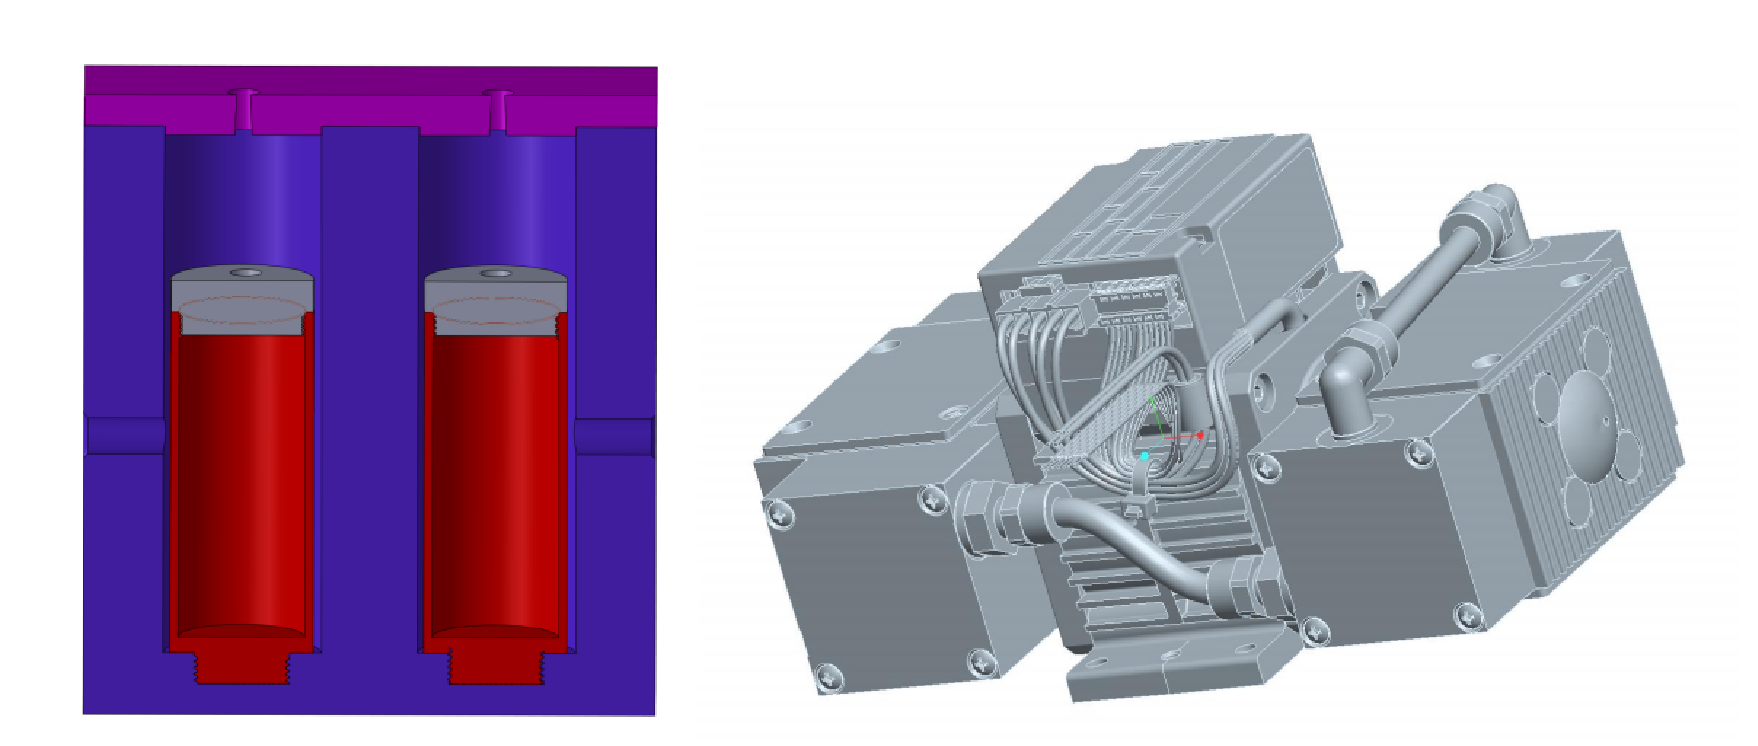
\includegraphics[width=0.5\textwidth]{figures/Astro_Figs.pdf}
		\caption{Clean Box with Containers and Pump.}
		\label{fig:Astro System}
	\end{center}
\end{figure}